\documentclass[a4paper]{article}
\usepackage[pdftex]{graphicx}
\usepackage[utf8]{inputenc}
\usepackage{enumerate}
\usepackage{icomma}
\usepackage{siunitx}
\sisetup{locale=DE} 
\usepackage{amssymb}
\usepackage{tikz}
\usepackage{href-ul}
\hypersetup{
	colorlinks=true,
	linkcolor=blue,
	urlcolor=blue}
\usepackage{geometry}
\geometry{a4paper, top=15mm, left=15mm, right=15mm, bottom=15mm,
	headsep=10mm, footskip=12mm}

\begin{document}
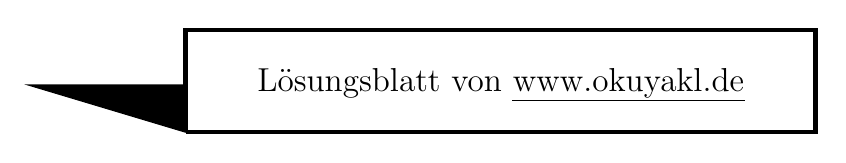
\begin{tikzpicture}(10,3)
	\draw[ultra thick](2,0) --(10,0) -- (10,1.3) --(2,1.3) -- (2,0);
	\draw[fill=black](2,0)-- (0,.6) -- (2,.6) -- (2,0);
	\node at (6,.6) {\large Lösungsblatt von \href{https://www.okuyakl.de}{www.okuyakl.de}};
\end{tikzpicture}
\vspace{0.5 cm}

\noindent{\bf Aufgabe 1.}\\
\begin{itemize}
	\item $\frac{e^2}{s}=g$: wahr (Kathetensatz)
	\item $ g^2 - e^2 = f^2 $: wahr (Satz des Pythagoras)
	\item $\frac{h^2}{s}=r$: wahr (Höhensatz) 
	\item $s^2=\sqrt{h^2-e^2}$: falsch; muss $s^2= e^2-h^2 $ heißen
\end{itemize}
\vspace{0.5 cm}

\noindent{\bf Aufgabe 2.}\\
Die Diagonale der Grundfläche ist:
$$ e =\sqrt{230^2 + 230^2} = \SI{325}{\meter}$$
Die Hälfte davon ist die Linie von einer Ecke zum Mittelpunkt. Wir wenden den Satz des Pythagoras an:
$$s = \sqrt{\left({e \over 2}\right)^2 + h^2}=\sqrt{163^2+140^2}=\SI{215}{\meter}$$
Die Seitenkante ist \SI{215}{\meter} lang.
\vspace{0.5 cm}
 
\noindent{\bf Aufgabe 3.}\\
Der Baum bildet ein Rechtwinkliges Dreieck mit den Katheten $a=5$; $b=x$ und der Hypotenuse $c=25-x$. Damit gilt:
$$
\renewcommand{\arraystretch}{2}
\begin{array}{rcll}
(25-x)^2 &=& 5^2 + x^2 \\
625 - 50x + x^2 &=& 25 + x^2 &|-x^2 + 50x -25\\
600 &=& 50x \\
x&=& \SI{12}{\meter}
\end{array}
$$
Der Baum ist in \SI{12}{\meter} Höhe abgeknickt.
\vspace{0.5 cm}

\noindent{\bf Aufgabe 4.}\\
Die längste Seite ist die Hypotenuse, somit stellen wir auf:
$$
\renewcommand{\arraystretch}{2}
\begin{array}{rcll}
c^2 &=& a^2 + b^2 \\
(4n^2+1)^2 &=& (4n^2-1)^2 + (4n)^2 \\
16n^4 + 8n^2 +1 &=& 16n^4 - 8n^2 +1 + 16n^2\\
              0 &=& 0 &(w)
\end{array}
$$
Wir erhalten eine wahre Aussage für alle $n \in \mathbb{R}$. Damit ist der Satz des Pythagoras immer erfüllt und die Dreiecke sind alle rechtwinklig. 
\vspace{0.5 cm}

\noindent{\bf Aufgabe 5.}\\
Wir bilden das rechtwinklige Dreieck $\Delta MDC$ mit $\overline{MC}=r=\SI{8}{\centi\meter}$.
Damit ist:
$$x=\overline{MD}=\sqrt{\overline{MC}^2-\overline{CD}^2}= \sqrt{8^2 - 4^2}=4\sqrt{3}=\SI{6,93}{\centi\meter}$$
\newpage

\noindent{\bf Aufgabe 6.}\\
Es sei die Breite $16x$ und die Höhe $9x$.
Dann erhalten wir:
$$\renewcommand{\arraystretch}{2}
\begin{array}{rcll}
70^2 &=& (16x)^2 + (9x)^2\\
4900 &=& 337x^2 &|:337\\
14,5 &=& x^2\\
3,8 &=& x \\
&\Rightarrow& \textnormal{Breite} =16\cdot 3,8&=\SI{61}{\centi\meter}\\
&\Rightarrow& \textnormal{Höhe} =9\cdot 3,8&=\SI{34}{\centi\meter}\\
\end{array}
$$
\begin{center}
	\includegraphics[width=7 cm]{../../viecher/endcomic.pdf}
	
	Hier geht es zurück zum \href{https://www.okuyakl.de/math/m9pyaL045/aa045.pdf}{Aufgabenblatt}
\end{center}

\end{document}

